%----------------------------------------------------------------------------
\chapter{\bevezetes}
%----------------------------------------------------------------------------
%----------------------------------------------------------------------------
\section{Rendszer modellezés}
%----------------------------------------------------------------------------

Napjainkban a modellezés fogalom nagyon elterjedté vált az ipari világ valamennyi ágában. A rendszermodellezés egy olyan folyamat, amelyben egy rendszert írunk le különböző absztrakciós szinteken. Minden modell egy különálló nézőpontból mutatja be a rendszert.

A modellek több nézőpontból írják le a rendszert:
 \begin{itemize}
 	\item Külső perspektíva, ahol a rendszer kontextusát és környezetét írjuk le
 	\item Belső perspektíva, ahol a rendszer belső komponensei közti és a környezettel való kapcsolatot írjuk le
 	\item Strukturális perspektíva, ahol a rendszer felépítését és a feldolgozott adatok struktúráját ábrázoljuk
 	\item Viselkedési perspektíva, ahol a rendszer viselkedését és különböző eseményekre való reakcióját részletezzük
 \end{itemize}

Mindehhez valamilyen grafikus jelölésre van szükségünk, a legismertebb ábrázolási szemantika a Unified Modeling Language (UML). Az öt legelterjedtebb UML diagram:
 \begin{itemize}
	\item Működési (Activity) - folyamatokat és adatfeldolgozási lépéseket modellezhetünk
	\item Használati eset (Use case) - a rendszer és a környezete közti interakciókat írjuk le
	\item Szekvencia (Sequence) - aktorok és rendszer továbbá belső komponensek közti kommunikációt ábrázolják
	\item Osztály (Class) - objektumokat és ezek közti hierarchikus kapcsolatokat tudjuk leírni
	\item Állapot (State) - a rendszer viselkedését modellezhetjük különböző belső vagy külső események hatására
\end{itemize}

%----------------------------------------------------------------------------
\section{Gamma keretrendszer}
%----------------------------------------------------------------------------
A Gamma keretrendszer (Gamma Állapotgép Kompozíciós Keretrendszer) egy olyan eszköz amivel komponens alapú reaktív rendszereket tudunk modellezni, verifikálni vagy akár kódot generálni. A gamma az egyetem Méréstechnika és Információs Rendszerek tanszékén készült, fő fejlesztője Graics Bence.

Reaktív rendszernek nevezzük azt az architekturális stílust, amely segítségével lehetőségünk van különálló alkalmazások egységként való kezelésére úgy, hogy ezek a komponensek továbbá képesek egymás eseményeire és a környezetükre reagálni.

A keretrendszer Yakindu (Yakindu Statechart Tools) alapokon készült, ami egy nyílt forráskódú állapotgépeket modellező eszköz. A gamma ezt továbbviszi és egy magasabb modellezési réteget biztosít a felhasználók számára, amely segítségével hierarchikus állapotgép hálózatokat tudnak kialakítani. A Gamma képes egyszerű állapotgépek és komplex állapotgép hálózatok modell verifikációjára, mindehhez felhasználja az UPAAL-t ami egy modell ellenőrző eszköz. Továbbá, a Gamma segítségével lehetőségünk van a teljes rendszerhez kódot generálni, jelenleg a Java nyelv támogatott.

%----------------------------------------------------------------------------
\section{Feladat áttekintés}
%----------------------------------------------------------------------------
Ahogy a modellalapú fejlesztési módszerek egyre elterjedtebbé válnak, úgy erősödik az igény a korszerűbb eszköztámogatásra is. Ennek egyik eleme, hogy az olyan funkciók mint pl. a kódgenerálás, modelltranszformációk, vagy modellellenőrzés a szoftverfejlesztésnél megszokott módon egy folytonos integrációs folyamat részét képezzék. Ráadásul ezen funkciók egy része igen erőforrásigényes, így adja magát az automatikusan skálázódó, felhőalapú szolgáltatások megjelenése is.


A Gamma egy Eclipse-alapú eszköz, így jelen formájában nem felel meg a fentebb vázolt modern követelményeknek. A feladat ennek megfelelően az, hogy az alkalmazás szolgáltatásként is használható részeit parancssoron keresztül, illetve OpenAPI segítségével webes szolgáltatásként is elérhetővé tegyük.

%----------------------------------------------------------------------------
\section{Motiváció}
%----------------------------------------------------------------------------

Ebbe a fejezetben részletezni fogom a feladatban említett felhő és webes szolgáltatások előnyeit.

%----------------------------------------------------------------------------
\subsection{Felhő alapú megoldások}
%----------------------------------------------------------------------------
Napjaikban egyre gyakrabban merül föl a Felhő/Cloud fogalom, ez annak köszönhető, hogy az informatika világában valamennyi kis- és nagyvállalat egyaránt vezet be különböző felhő alapú szolgáltatásokat. Három fő kategóriába tudjuk csoportosítani a felhőalapú szolgáltatásokat:

\begin{enumerate}
	\item \textbf{Software as Service (SaaS)} leggyakrabban használt megoldás, alkalmazások disztribúciója az interneten keresztül felhasználók számára
	\item \textbf{Infrastructure as Service (IaaS)}	Skálázható és automatizált erőforrások
	\item \textbf{Platform as Service (PaaS)} Olyan környezetet biztosít a fejlesztők számára, amelyen kényelmesen tudnak alkalmazásokat fejleszteni
\end{enumerate}

Számos előnyei vannak a fenti felhő alapú szolgáltatásoknak, 3 fő kategóriába tudjuk ezeket sorolni:

 \begin{itemize}
	\item \textbf{Flexibilitás} : Igény szerint skálázható, publikus és privát adattárolás lehetősége, vezérlési lehetőségek (egy szervezet eldöntheti, hogy milyen szinten szeretné kontrollálni az igényelt szolgáltatását), gazdag portfólió (számos létező eszköz és megoldás közül választhatunk) és nem utolsó sorban biztonsági szempontból is rengeteg létező vagy új megoldást lehet implementálni az adatok titkosításához
	\item \textbf{Hatékonyság} : Elérhetőség - bárhonnan elérhető egy szolgáltatás az interneten keresztül, idő megtakarítás szempontjából fejlesztők gyorsabban tudnak dolgozni, Hardware biztonság - egy esetleges hardware meghibásodás során nem veszítünk adatokat, anyagi megtakarítás - vállalatoknak nincs szüksége szerverekre és más hasonló felszerelésre
	\item \textbf{Stratégiai érték} : Számos terhet vesz le egy felhőalapú szolgáltatás a szervezetek válláról, így több idő marad a fejlesztésekre, mindig friss az igénybe vett szolgáltatás verziója. Az elérhetőség lehetővé teszi, hogy a világ bármilyen részéről emberek közösen tudjanak dolgozni ugyanazon a problémán
\end{itemize}

%----------------------------------------------------------------------------
\subsection{Webes szolgáltatások}
%----------------------------------------------------------------------------

Egy webes szolgáltatás lehetővé teszi, hogy a meglévő szoftverünket elérhetővé tegyük a világ számára. HTTP protokollt használva nem csak kliensek felé oszthatjuk meg, hanem különböző más létező szoftver komponensekkel való kommunikációt is kitudunk alakítani.

Számos előnye van: Rengeteg már létező megoldás van már belőle, így nehéz elakadni. Jól előredefiniált protokollok lettek meghatározva, így bármilyen szoftveres világ tud kommunikálni egy teljesen más világgal.

%----------------------------------------------------------------------------
\section{Megoldás}
%----------------------------------------------------------------------------
A fentebb leírtak alapján a Gamma egy Eclipse IDE-n belüli eszköz, ennek a transzformációját webes szolgáltatásba a következő ábra írja le:

\begin{figure}[!ht]
	\centering
	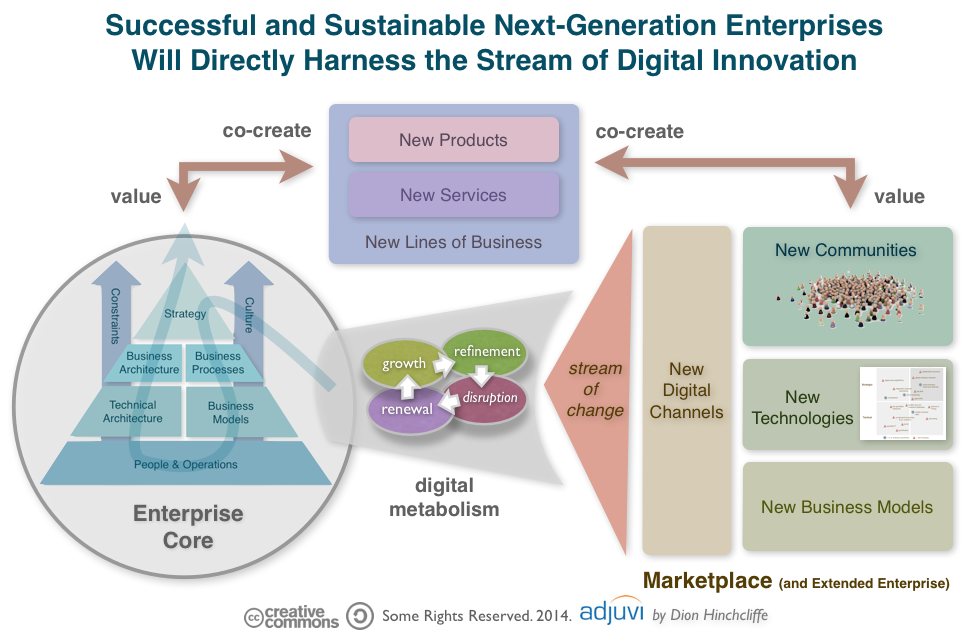
\includegraphics[width=150mm, keepaspectratio]{figures/place_holder1.png}
	\caption{Gamma infrastruktúra}
	\label{fig:TeXstudio}
\end{figure}


Alapvetően a Gammát mint Eclipse IDE Plug-in ki kellet emelni, hogy egy fekete szoftver doboz legyen, ami bemeneti paraméterként kap egy műveleteket leíró fájlt, ezután legyártja a különböző műveletek által definiált eredmény fájlokat. A gamma fölé kellet építeni egy webes kiszolgálót, ami képes bejövő kéréseket értelmezni, majd átfogalmazva tovább küldi a Gamma komponensnek. A megoldás során olyan mellék/segítő komponenseket is megkellet tervezni és implementálni, amelyek az adatok átalakításáért vagy mozgatásáért felelősek.
%----------------------------------------------------------------------------
\section{Dolgozat felépítése}
%----------------------------------------------------------------------------

A szakdolgozat keretin belül a fentebb leírt megoldás specifikációját, fejlesztési folyamatát, tesztelési útmutatóját és továbbfejlesztési lehetőségét részletezem.

A következő fejezetben bemutatom az általam választott technológiákat amelyekkel a feladatot megoldottam, itt bemutatásra kerülnek a OSGi, Eclipse RCP, REST API stb. fogalmak. Továbbá, a feladatot specifikálni fogom, megfogalmazott követelményeket mutatok be és végigvezetem a fejlesztési folyamaton és felmerülő nehézségek megoldásában az olvasót. Ezt követően bemutatom a fejlesztést egy konkrét példa segítségével, zárásként pedig a továbbfejlesztési lehetőségekről fogok beszámolni.





















